\begin{figure}[t]
    \centering
    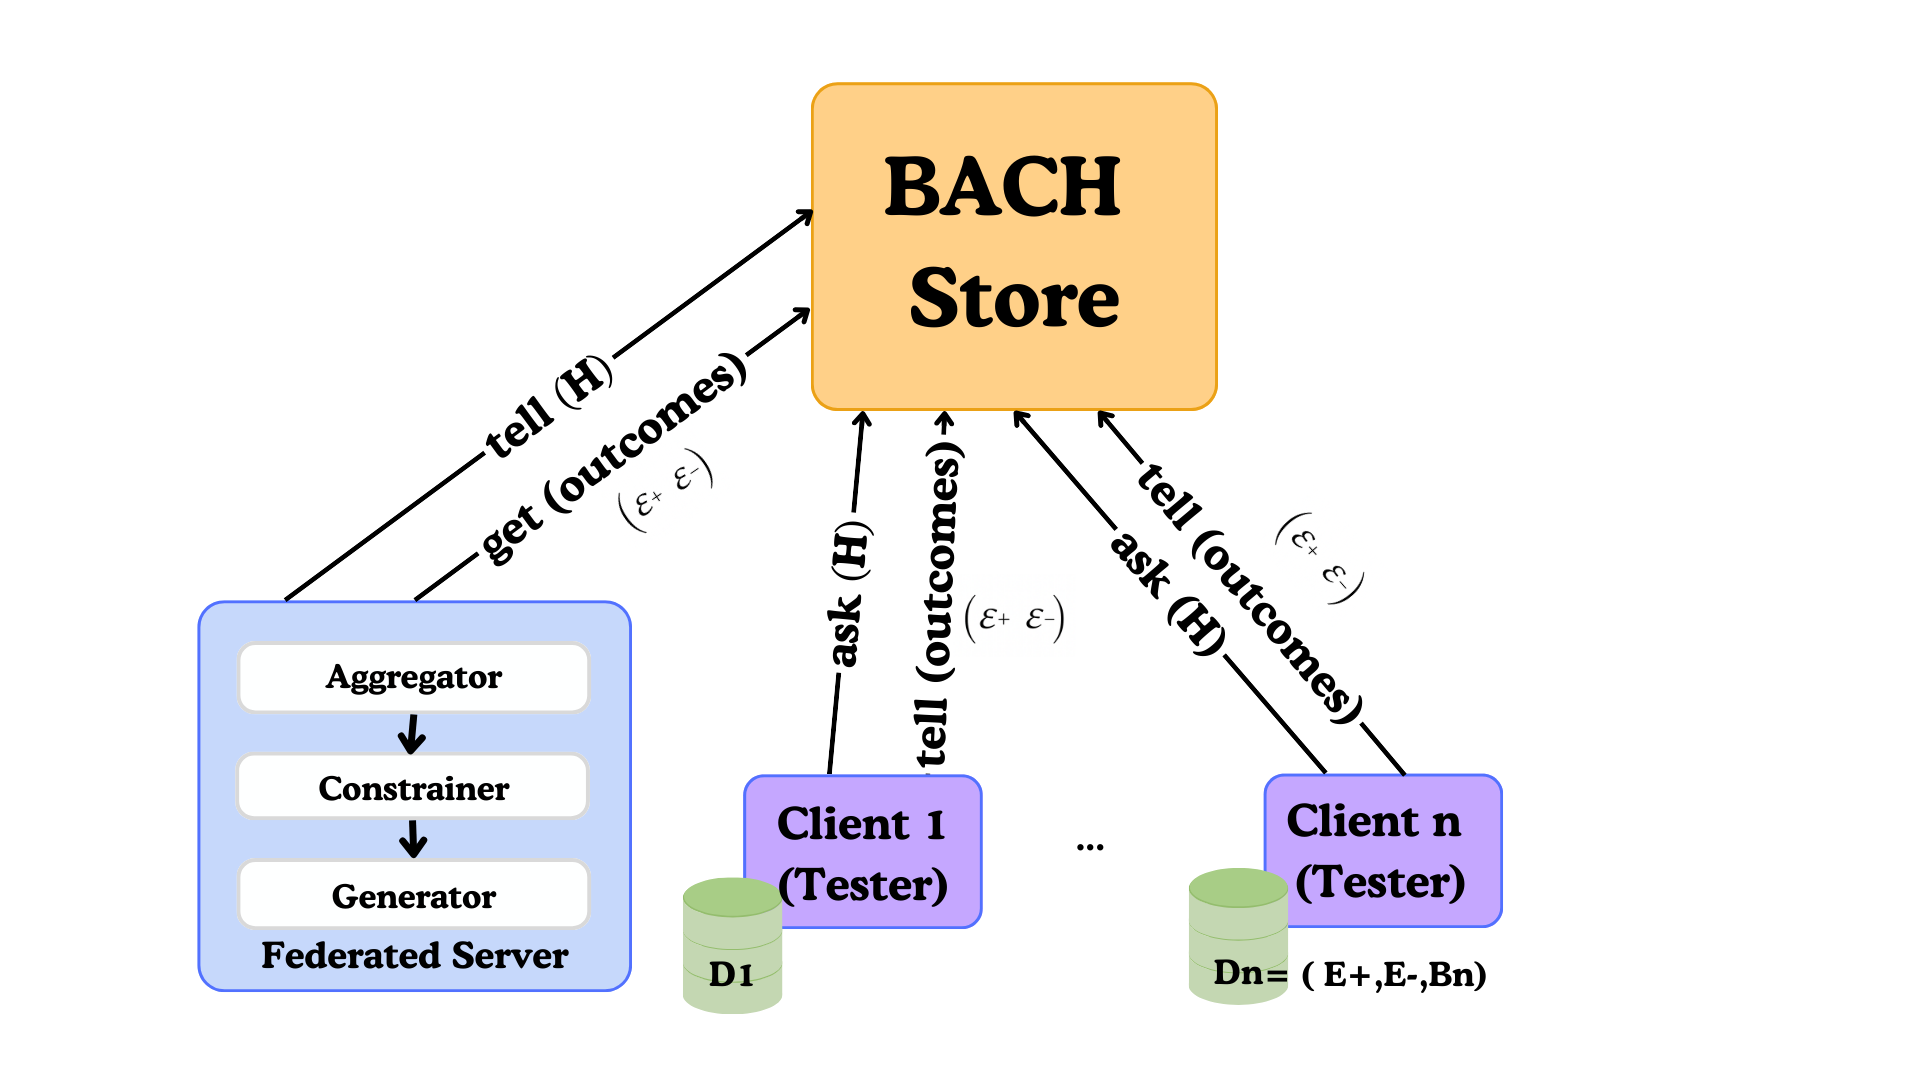
\includegraphics[width=\linewidth]{bach-popper.png}
    \caption{BACH4Popper Architecture (A Yasmine, refaire le dessin pour tenir compte de la signification des lettres (à discuter à la rentrée))}
    \label{fig:bachpopper}
\end{figure}

\section{The Bach4Popper Framework}
\label{sect-BachForPopper}

\subsection{The framework}

We are now in a position to explain how to implement federated inductive logic programming using Popper and BLPy. As illustrated in
Figure~\ref{fig:bachpopper}, given the store made available by BLPy, the basic idea
is to have a BLPy server process, named \texttt{bbpopper}, handling the store,
and two types of BLPy client processes communicating through it. One of them,
referred to as \texttt{srvpopper}, is deployed in a unique
instance. It is responsible for the generate and constraint parts of
Algorithm~\ref{alg:popper}. The other types of clients, named
\texttt{clipopper}, are deployed in as many instances as data entities
available. They are responsible for the test part of
Algorithm~\ref{alg:popper} on their local data.  The two types of
clients communicate via the store. It is assumed that the number of
\texttt{clipopper} clients are known in advance, that
\texttt{clipopper} clients are identified by numbers ranging from $1$
to this number, and that no intruder modifies the content of the
store. 

% These hypotheses are discussed in
% Subsection~\ref{sub-extensions}. Before that, we first describe in
% more details the algorithms behind \texttt{srvpopper} and
% \texttt{clipopper} clients and establish that the resulting federated
% version of Popper is equivalent to the centralized version of Popper,
% defined in Section~\ref{section-popper}.



%Basically, from a coordination perspective, the \texttt{srvpopper} client iteratively tells the current hypothesis on the store, asks for the confusion matrices returned by \texttt{clipopper} clients, aggregates them and computes new constraints. 

Basically, from a coordination perspective, the \texttt{srvpopper} process iteratively publishes the current hypothesis to the shared store and queries the local evaluation feedback produced by the \texttt{clipopper} clients. Each client evaluates the hypothesis locally and returns symbolic feedback derived from its confusion matrix. The server aggregates these feedbacks, computes new logical constraints, and uses them to refine the hypothesis. 
%Algorithm~\ref{alg:srvpopper} provides the precise instructions. It is based on Algorithm~\ref{alg:popper}.

\begin{algorithm}[t]
  \caption{Srvpopper client}
  \label{alg:srvpopper}
  \small
  \begin{lstlisting}
def srvpopper(N, D, C, max_vars, max_literals, max_clauses):

    CC = C
    best_score = 0
    best_hyp = { }
    end_popper = false
    num_literals = 0
    r = 1

    while not end_popper and num_literals <= max_literals:
       c_solvable = true
       num_literals += 1
       while not end_popper and c_solvable:
          hyp = generate(D, CC, max_vars, num_literals, max_clauses)
          if not hyp:
             c_solvable = false
          else:
             tell(hypsi(r,hyp))
             for i in range(1,N+1):
                cm[i] = ask(cmtuple(r,i))
             outcome = aggregate_outcome(cm)
             score = aggregate_score(cm)
             if outcome == ('all', 'none'):
                best_hyp = hyp
                end_popper = true
                tell(hypsi(r,nil_hyp))                
             else:
                if best_score < score:
                   best_hyp = hyp
                   cc += learn_constraints(hyp, outcome)
           r = r+1
                   
    return best_hyp
  \end{lstlisting}
\end{algorithm}



Algorithm~\ref{alg:srvpopper} details the server-side learning procedure and is directly derived from Algorithm~\ref{alg:popper}.
It uses the function \texttt{srvpopper} function as the main function. The prototype is the same as the one of function \texttt{popper} in Algorithm~\ref{alg:popper} except that the argument $B$ providing the background knowledge is omitted. %This argument is indeed distributed on the \texttt{clipopper} processes. 
This omission reflects the fact that background knowledge is locally available on the distributed \texttt{clipopper} processes.
%The instructions of the initialisation are the same, except for the introduction of an integer variable \texttt{r} which provides a counter for the current round in the Popper generate-test-constraint cycle. 

The initialization phase follows the same structure as in centralized Popper, with the addition of an integer variable \texttt{r} that tracks the current federated round in the generate–test–constrain cycle.

The two loops of Algorithm~\ref{alg:popper} are also essentially repeated, with the following differences. Instead of calling the \texttt{test} function to determine the confusion matrix, the current hypothesis (in case it exists) is told via the execution of the \texttt{tell(hypsi(r,hyp))} primitive. Then the \texttt{srvpopper} process waits for the confusion matrices computed by the \texttt{clipopper} processes by means of the execution of the \texttt{ask(cmtuple(r,i))}, the result being stored in an array \texttt{cm}. Each element of this array reflects the result of a local computation, which is then aggregated by the \texttt{aggregate\_outcome} and \texttt{aggregate\_score} functions. The end of the execution is then similar to the one of function \texttt{popper}, with as two differences that the end of the execution is reported by telling an empty hypothesis by the primitive \texttt{tell(hypsi(r,end\_hyp))} and that each iteration ends by updating the \texttt{r} counter. The precise definitions of the \texttt{aggregate\_outcome} and \texttt{aggregate\_score} functions is specified in Definition~\ref{def-aggregation} when theoretical results will make clear what they should be.


\mytodo{JMJ: add a paragraph on aggregation}




\medskip
A \texttt{clipopper} client, say identified by $I$, executes dually. Basically it  
iterates by asking for the current hypothesis, tests it on its local
data $E_I^+$, $E_I^-$, $B_I$, computes the confusion matrix and tells it. This is operated by function \texttt{clipopper} of Algorithm~\ref{alg:clipopper}.

\begin{algorithm}[t]
  \caption{Clipopper client}
  \label{alg:clipopper}
  \small
  \begin{lstlisting}
def clipopper(I, EI+, EI-, BI):

       end_popper = false
       r = 1

       while not end_popper:
          hyp_asked = ask(hypsi(r))
          if (hyp_asked = hyp(r,end_hyp):
             end_popper = true
          else:
             conf_matrix = test(EI+, EI-, BI, hyp_asked)
             tell(cmtuple(r,Id,conf_matrix)
          r = r+1

  \end{lstlisting}
\end{algorithm}




\subsection{Theoretical results}

As a summary of the previous subsection, by identifying the processes with their main function and by keeping the maximum number of variables, literals and clauses as local data of the Popper server, the federated computation consists in executing the following parallel agent:
%
\begin{eqnarray}
FedPopper(N) & = & \begin{array}[t]{l}
                     bbpopper || srvpopper(N, D, C) || \\
                     clipopper(1,E_1^+,E_1^-,B_1) || ... || 
                     clipopper(N,E_N^+,E_N^-,B_N)
                    \end{array}
\label{eqn-FedPopper}               
\end{eqnarray}

We now have to establish that the final hypothesis computed by this execution is the same as the one computed by function \texttt{popper} of Algorithm~\ref{alg:popper}. This is obviously only possible if a relation is identified between positive and negative examples, on the one hand, as well as the background knowledge, on the other hand. This is precisely the aim of the following definition.

\begin{definition}
Let $E$ be a set of ground atoms. The set $U(E)$ is defined as the set of ground terms formed from constants and functions appearing in the arguments of atoms of $E$. By extension, if $E^+$ and $E^-$ are sets of positive and negative examples on a predicate $p$, the set $U(E^+,E^-)$ is defined as $U(E^+) \cup U(E^-)$.
\end{definition}

\begin{definition}
 A Horn clause program $B$ is said to be well-structured if it can be partitioned into a set $SF$ of facts and a set of definite Horn clauses $SH$ whose literal arguments are variables and whose head does not involve predicate of $SF$. Such a partition is unique by construction. The two sets are respectively referred to as
 $sf(B)$ and $sh(B)$, respectively.
\end{definition}

\begin{definition}
Let $E^+, E_1^+, \cdots, E_n^+$ and $E^-, E_1^-, \cdots, E_n^-$ be respectively sets of positive and negative examples on a predicate $p$. Let $B, B_1, \cdots, B_n$ be well-structured Horn clause programs. The set 
\( \{ (B_1, E_1^+,E_1^-), \cdots, (B_n, E_n^+,E_n^-) \}
\)
is a federated partition of $(B, E^+,E^-)$ iff the following conditions hold:

\begin{itemize}
\item $U(sf(B_i)) \subseteq U(E_i^+,E_i^-)$, for any $i=1, \cdots, n$
\item $sf(B_1) \cdots, sf(B_n)$ form a partition of $sf(B)$
\item the sets $U(E_i^+,E_i^-)$ and $U(E_j^+,E_j^-)$ are disjoint, for any 
      $i,j=1, \cdots, n$ with $i \not= j$
\item one has $sh(B_1) = \cdots = sh(b_n) = sh(B)$
\item $E_1^+, \cdots, E_n^+$ form a partition of $E^+$
\item $E_1^-, \cdots, E_n^-$ form a partition of $E^-$
\end{itemize}
\end{definition}

\begin{proposition}
\label{key-prop-pos}
Let \( \{ (B_1, E_1^+,E_1^-), \cdots, (B_n, E_n^+,E_n^-) \}
\)
be a federated partition of $(B, E^+,E^-)$ with positive and negative examples over the predicate $p$. Let $H$ be a Horn clause program. Then for any $e^+ \in E^+$, one has  \( \jmjderiv{B \cup H}{\mfm{e^+}}{\theta} \) iff 
\( \jmjderiv{B_i \cup H}{\mfm{e^+}}{\theta} \) for some $i=1, \cdots, n$.
\end{proposition}


\begin{proof}
Assume first that \( \jmjderiv{B \cup H}{\mfm{e^+}}{\theta} \). Then there exists a derivation $Deriv$ from $e^+$ using clauses of $B \cup H$ ending with the empty clause and producing $\theta$ as computed answer substitution. This derivation uses clauses of $H$, $sh(B)$ and facts from $sf(B)$. As $E_1^+, \cdots, E_n^+$ form a partition of $E^+$ there exists one and only one $i$ such that $e^+ \in E_i^+$. In view of the federated partition assumption, the set of the facts used in $Deriv$ are then included in $sf(B_i)$. As the Horn clauses of $sh(B_i)$ are those of $sh(B)$, it follows that the derivation $Deriv$ is also a derivation establishing that \( \jmjderiv{B_i \cup H}{\mfm{e^+}}{\theta} \). 

Assume now that  \( \jmjderiv{B_i \cup H}{\mfm{e^+}}{\theta} \), for some $i$. There is thus a derivation from $e^+$ using clauses of $B_i \cup H$ ending with the empty clause and producing $\theta$ as computed answer substitution. As $sh(B_i) = sh(B)$ and $sf(B_i) \subseteq sf(B)$, this derivation is also a derivation using clauses of $B \cup H$. It follows that \( \jmjderiv{B \cup H}{\mfm{e^+}}{\theta} \).
\end{proof}

As a direct consequence, any $e^- \in E^-$ is not derivable from $B \cup H$ if it is not derivable from $B_i \cup H$ for any $i$. However, the federated partition property allows to go one step further.

\begin{proposition}
\label{key-prop-neg}
Let \( \{ (B_1, E_1^+,E_1^-), \cdots, (B_n, E_n^+,E_n^-) \}
\)
be a federated partition of $(B, E^+,E^-)$ with positive and negative examples over the predicate $p$. Let $H$ be a Horn clause program. Let $e^-$ be a negative example of $E^-$. It is thus a negative example of some $E_j^-$. Then $E^-$ is not derivable from $B \cup H$ iff it is not derivable from $B_j \cup H$.
\end{proposition}

\begin{proof} 
Indeed, in view of the federated partition assumption, 
$U(sf(B_j)) \subseteq U(E_j^+,E_j^-)$ and the sets 
$U(E_k^+,E_k^-)$ are disjoint. Therefore checking whether 
\( \jmjderiv{B \cup H}{\mfm{e^+}}{\theta} \)
holds amount to checking whether
\( \jmjderiv{B_j \cup H}{\mfm{e^+}}{\theta} \)
hold. 
\end{proof}


It follows from propositions~\ref{key-prop-pos} and \ref{key-prop-neg} that the 
confusion matrix computed (centrally) on $(B,E^+,E^-)$ consists of the component-based sum of the confusion matrices computed (locally) for the $(B_i,E^+_i,E^-_i)$.

\begin{proposition}
\label{prop-conf-matrices}
Let \( \{ (B_1, E_1^+,E_1^-), \cdots, (B_n, E_n^+,E_n^-) \}
\)
be a federated partition of $(B, E^+,E^-)$ with positive and negative examples over the predicate $p$. Let $H$ be a Horn clause program. Let 
$(TP,FN,TN,FP)$ be the confusion matrix for $H$ determined with respect to $(B, E^+,E^-)$. For any $i=1, \cdots, n$, let $(TP_i,FN_i,TN_i,FP_i)$ be the confusion matrix for $H$ determined with respect to $(B_i, E_i^+,E_i^-)$. Then 
\[ \begin{array}{lcl}
TP = \sum_{i=1}^{n} TP_i    & \hspace*{2ex} & TN = \sum_{i=1}^{n} TN_i \\
FP = \sum_{i=1}^{n} FP_i    & \hspace*{2ex} & FN = \sum_{i=1}^{n} FN_i
\end{array} \]
\end{proposition}

\begin{proof}
Direct consequence of propositions~\ref{key-prop-pos} and \ref{key-prop-neg}
\end{proof}

This result allows for a direct aggregation of confusion matrices. However the confusion matrix is not used as such to determine new constraints but through the outcome and score only, it is possible to go one step further. Before that, let us define an aggregation of outcome and score as follows.

\begin{definition}
Define 
\(\oplus : \{ \mathit{all}, \mathit{some}, \mathit{none} \}
              \times 
              \{ \mathit{all}, \mathit{some}, \mathit{none} \}
              \rightarrow
              \{ \mathit{all}, \mathit{some}, \mathit{none} \}
\)
as follows:
\begin{eqnarray*}
    o_1 \oplus o_2 = \left\{\begin{array}{ll}
                             \mathit{all} & \mbox{if } o_1 = o_2 = \mathit{all} \\
                             \mathit{none} & \mbox{if } o_1 = o_2 = \mathit{none} \\
                             \mathit{some} & \mbox{otherwise}
                           \end{array}
                     \right.
\end{eqnarray*}
\end{definition}

It is easy to verify that the operator $\oplus$ is commutative and associative. This allows to state the following proposition.

\begin{proposition}
\label{prop-agg}
Let \( \{ (B_1, E_1^+,E_1^-), \cdots, (B_n, E_n^+,E_n^-) \}
\)
be a federated partition of $(B, E^+,E^-)$ with positive and negative examples over the predicate $p$. Let $H$ be a Horn clause program. Let 
$(po,no)$ and $s$ be respectively the outcome and score computed for $H$ with respect to $(B, E^+,E^-)$. For any $i=1, \cdots, n$, let $(po_i,no_i)$ and $s_i$ be respectively the outcome and score computed for $H$ with respect to $(B_i, E_i^+,E_i^-)$. Then 
\begin{eqnarray*}
    po & = & po_1 \oplus \cdots \oplus po_n \\
    no & = & no_1 \oplus \cdots \oplus no_n \\
    s  & = & s_1 + \cdots + s_n
\end{eqnarray*} 
\end{proposition}

\begin{proof}
The proposition directly follows from proposition~\ref{prop-conf-matrices}.
\end{proof}

The correctness of the federated computation embodied in equation~\ref{eqn-FedPopper} and algorithms~\ref{alg:srvpopper} and \ref{alg:clipopper} with respect to the central computation embodied in algorithm~\ref{alg:popper} then comes from the fact that hypotheses $hyp$ successively computed by algorithm~\ref{alg:popper} and those that are successively told in algorithm~\ref{alg:srvpopper}. This is easily established by induction, as thanks to proposition~\ref{prop-agg}, the outcome and score computed in a distributed manner are exactly those computed in a centralized way and thus induce the same constraints to be used in a generation phase.


\subsection{Experiments}

Yasmine : deux types d'expérimentations à faire svp

\begin{itemize}

\item superposer Algos 1 et 2 en un algorithm 4 (cf algo ci-arpès) et vérifier qu'à chaque itération, ce qui est calculé globalement est le même que ce qui est calculé de manière fédérée

\item faire tourner Algo 1 de nombreuses fois (par exemple 100 fois) sur chacun des exemples et de même de manière fédérée et comparer les temps d'exécution. Idéalement ils devraient être les memes.

\end{itemize}


\begin{algorithm}[t]
  \caption{Popper + Srvpopper client pour tests de Yasmine}
  \label{alg:srvpopper}
  \small
  \begin{lstlisting}
def g_and_srvpopper(N, E+, E-, B, D, C, max_vars, max_literals, max_clauses):

    CC = C
    best_score = 0
    best_hyp = { }
    end_popper = false
    num_literals = 0
    r = 1

    while not end_popper and num_literals <= max_literals:
       c_solvable = true
       num_literals += 1
       while not end_popper and c_solvable:
          hyp = generate(D, CC, max_vars, num_literals, max_clauses)
          if not hyp:
             c_solvable = false
          else:
             // execution globale
             conf_matrix = test(E+, E-, B, hyp)
             outcome_g = compute_outcome(conf_matrix)
             score_g = compute_score(conf_matrix)
            // execution federee
             tell(hypsi(r,hyp))
             for i in range(1,N+1):
                cm[i] = ask(cmtuple(r,i))
             outcome_fed = aggregate_outcome(cm)
             score_fed = aggregate_score(cm)
             // comparaison des resultats
             if (outcome_g != outcome_fed) || (score_g != score_fed):
                 print("Calcul global non consistant avec calcul federe !")
             if outcome == ('all', 'none'):
                best_hyp = hyp
                end_popper = true
                tell(hypsi(r,nil_hyp))                
             else:
                if best_score < score:
                   best_hyp = hyp
                   cc += learn_constraints(hyp, outcome)
           r = r+1
                   
    return best_hyp
  \end{lstlisting}
\end{algorithm}


\subsection{Extensions}
